% !TEX root = main.tex
\documentclass[10pt, a4paper]{article}

% ── Packages ──────────────────────────────────────────────────────────────────
\usepackage[
  top=0.35in, bottom=0.35in,
  left=0.45in, right=0.45in
]{geometry}
\usepackage[dvipsnames]{xcolor}
\usepackage{hyperref}
\usepackage{graphicx}
\usepackage{titlesec}
\usepackage{enumitem}
\usepackage{array}
\usepackage{tabularx}
\usepackage{parskip}

% ── Hyperlink styling ─────────────────────────────────────────────────────────
\hypersetup{
  colorlinks=true,
  urlcolor=black,
  linkcolor=black
}

\pagestyle{empty}

% Section formatting
\titleformat{\section}
  {\normalsize\bfseries}
  {}{0em}{\MakeUppercase}
  [\vspace{-6pt}\rule{\linewidth}{0.5pt}]

\titlespacing{\section}{0pt}{6pt}{2pt}

\setlist[itemize]{noitemsep, topsep=0pt, partopsep=0pt, parsep=0pt, leftmargin=1.2em, itemsep=0pt}

\setlength{\parindent}{0pt}
\setlength{\parskip}{0pt}

% Set base font size slightly larger than 10pt default
\fontsize{10.5}{13.5}\selectfont

% ══════════════════════════════════════════════════════════════════════════════
\begin{document}

% ── HEADER ────────────────────────────────────────────────────────────────────
\noindent
\begin{minipage}[c]{0.48\textwidth}
  \raggedright
  {\fontsize{24}{28}\selectfont \textbf{YOUR NAME}}\par
  \vspace{3pt}
  {\large\itshape\color{gray} Systems Engineer $|$ Rust \& Go $|$ High-Performance Applications}\par
\end{minipage}%
\hfill
\begin{minipage}[c]{0.36\textwidth}
  \raggedleft
  \begin{minipage}[c]{0.68\linewidth}
    \raggedleft
    {\small\itshape\color{gray}
      \href{mailto:your.email@example.com}{your.email@example.com}\\[3pt]
      +91\,00000\,85302\\[3pt]
      \href{https://linkedin.com/in/your-linkedin}{linkedin.com/in/your-linkedin}\\[3pt]
      \href{https://github.com/your-github}{github.com/your-github}\\
    }
  \end{minipage}%
  \hspace{0.1pt}
\begin{minipage}[c]{0.26\linewidth}
    \raggedleft
    \fboxsep=2pt\fboxrule=0.5pt
    \fbox{%
      \IfFileExists{../assets/profile-photo.jpg}{%
        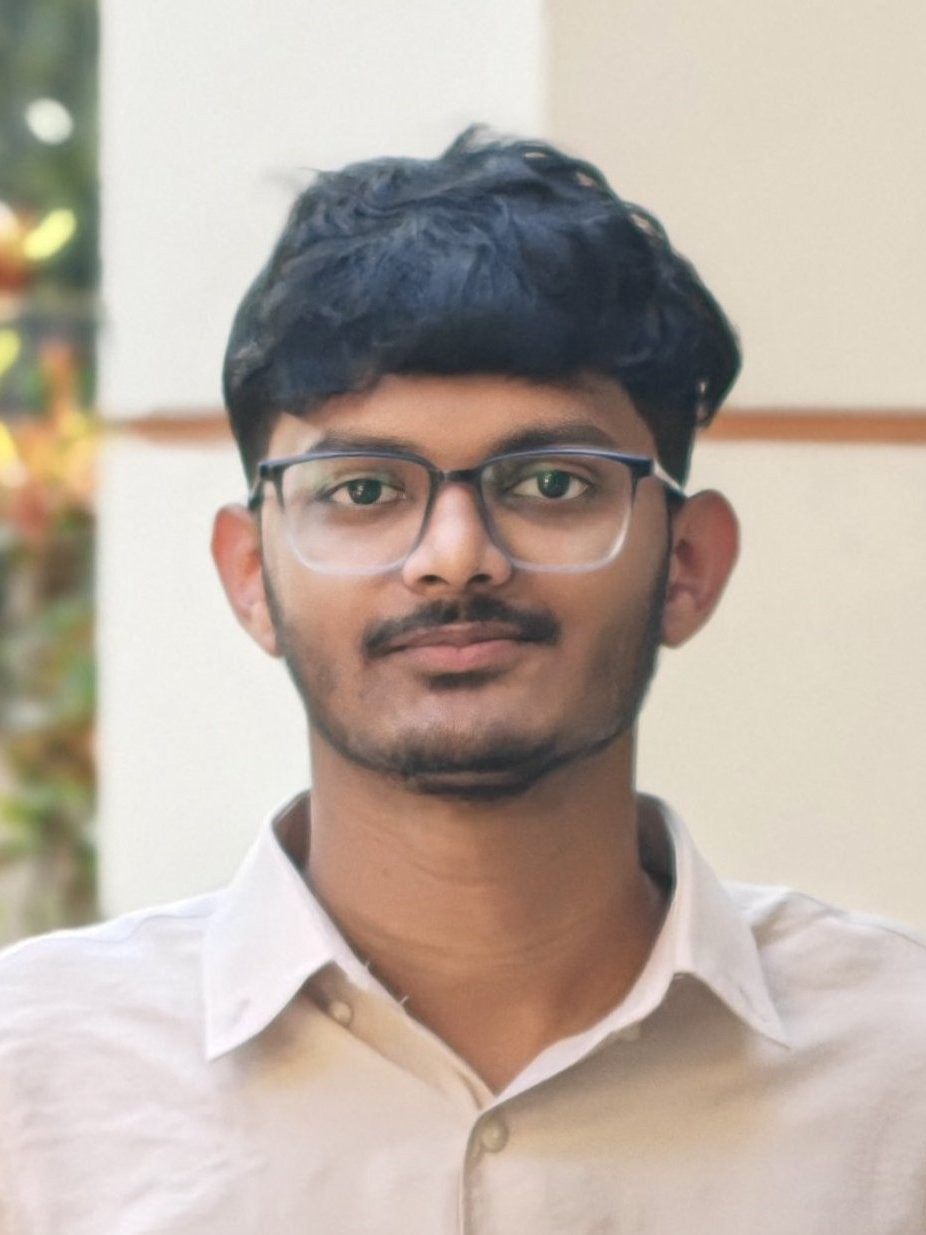
\includegraphics[height=0.75in,keepaspectratio]{../assets/profile-photo.jpg}}{%
      \IfFileExists{../assets/profile-photo.png}{%
        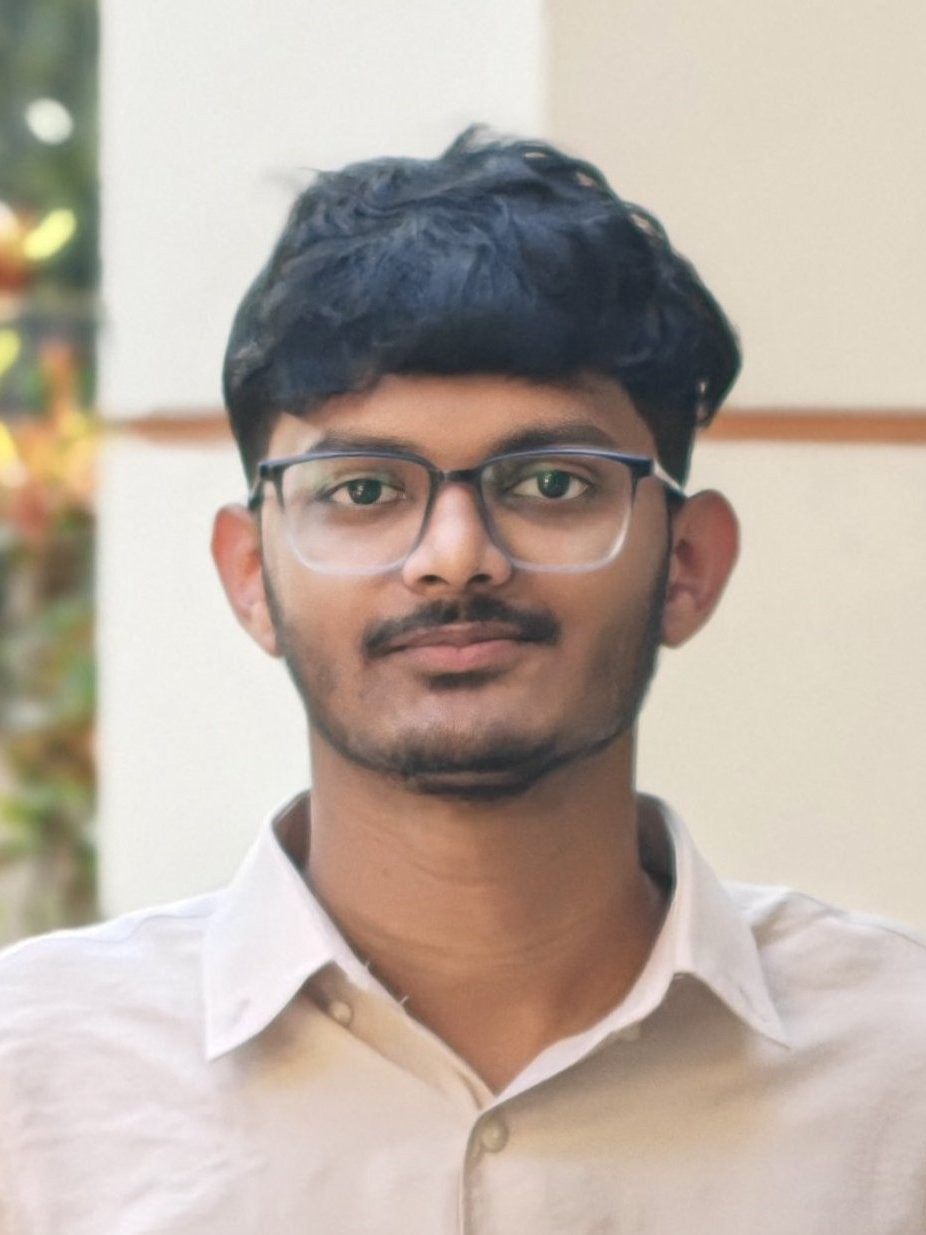
\includegraphics[height=0.75in,keepaspectratio]{../assets/profile-photo.png}}{%
      \IfFileExists{../assets/photo.jpg}{%
        \includegraphics[height=0.75in,keepaspectratio]{../assets/photo.jpg}}{%
      \IfFileExists{../assets/photo.png}{%
        \includegraphics[height=0.75in,keepaspectratio]{../assets/photo.png}}{}}}}%
    }%
  \end{minipage}
\end{minipage}

% ── CONTENT ──────────────────────────────────────────────────────────────────
\section*{Objective}

Systems-focused developer with experience in Rust and Go, building high-performance desktop and backend applications. Optimized execution speed by up to 40\% and reduced memory footprint. Focused on low-level optimization and efficient resource utilization, leveraging Rust’s memory safety model.

%------------------------------------------------------------
% TECHNICAL SKILLS
%------------------------------------------------------------
\section*{Skills}

\renewcommand{\arraystretch}{1.05}
\begin{tabular}{@{} >{\bfseries}p{3.8cm} p{13cm} @{}}
Languages           & Rust, Go, C, Python, JavaScript, Java \\
Systems/Performance & Concurrency, Memory Optimization, Native Binary Optimization \\
Frameworks          & Tauri, Wails, Flask, Node.js \\
Tools               & Git, GitHub Actions, Docker, ADB \\
Infrastructure      & DigitalOcean, Cloudflare \\
Operating Systems   & Linux, Windows, Win32 API Interop \\
\end{tabular}

%------------------------------------------------------------
% PROJECTS
%------------------------------------------------------------
\section*{Projects}

\textbf{DroidOps -- Android Device Management GUI} \hfill \textit{Tauri, React, Rust, TypeScript \quad Dec 2025} \quad \href{https://github.com/your-github/droidops}{[GitHub]}
\begin{itemize}
\item Engineered a Rust-based ADB management system using Tauri, improving process execution efficiency by 40\%.
\item Optimized native command execution pipeline, reducing manual operation latency and improving discovery speed.
\item Leveraged Rust's concurrency model to handle multi-device synchronization with near-zero overhead.
\end{itemize}

\vspace{3pt}

\textbf{GlyphDeck -- Desktop Font Manager} \hfill \textit{Go, TypeScript, Wails \quad Nov 2025} \quad \href{https://github.com/your-github/GlyphDeck}{[GitHub]}
\begin{itemize}
\item Built a high-performance Go application indexing 1,200+ fonts with sub-500ms retrieval latency.
\item Optimized memory footprint, achieving a lightweight \textasciitilde25MB native executable using Wails framework.
\item Enhanced user productivity by 40\% through optimized search algorithms and efficient font metadata parsing.
\end{itemize}

\vspace{3pt}

\textbf{AI-Based Smart Traffic System Using Computer Vision} \hfill \textit{Python, YOLO, Flask \quad Jan 2025}
\begin{itemize}
\item Implemented a YOLO-v8 based detection pipeline with 94\% accuracy in diverse conditions.
\item Optimized model inference for real-time edge operation, ensuring low-latency scene analysis ($<$200ms).
\item Developed adaptive signal control logic, reducing simulated intersection wait times by 25\%.
\end{itemize}

\vspace{3pt}

\textbf{IRRIGO -- Smart Irrigation Platform} \hfill \textit{Next.js, Flask, Python, REST APIs \quad Oct 2024}
\begin{itemize}
\item Developed an AI-driven backend integrating satellite data for high-accuracy water scheduling.
\item Analyzed 50+ farm scenarios to optimize resource allocation, projecting 20\% wastage reduction.
\item Engineered a real-time analytics dashboard via optimized RESTful APIs.
\end{itemize}

\vspace{3pt}

\textbf{Certificate Generator and Verification System} \hfill \textit{Node.js, Firebase, EJS, Tailwind \quad Dec 2024}
\begin{itemize}
\item Automated bulk certificate generation for 5,000+ records, reducing issuance effort by 90\%.
\item Implemented QR-based verification enabling 100\% instant credential validation via secure web links.
\item Engineered an interactive canvas editor using draggable and customizable layouts.
\end{itemize}

%------------------------------------------------------------
% EDUCATION
%------------------------------------------------------------
\section*{Education}

\textbf{B.Tech in Computer Science and Engineering} \hfill \textbf{2022 -- 2026}\\
Mar Baselios Christian College of Engg. \& Tech., Kuttikkanam \hfill APJ Abdul Kalam Technological University

%------------------------------------------------------------
% CERTIFICATIONS
%------------------------------------------------------------
\section*{Certifications}

\renewcommand{\arraystretch}{1.1}
\begin{tabular}{@{} p{7.8cm} p{6.5cm} p{2.5cm} @{}}
\textbf{Certificate}                  & \textbf{Issuer}              & \textbf{Year} \\[1pt]
Programming with Python               & Python Institute (OpenEDG)   & 2024 \\
Ubuntu Linux Professional Certificate & Canonical                    & Nov 2025 \\
\end{tabular}

%------------------------------------------------------------
% ACHIEVEMENTS
%------------------------------------------------------------
\section*{Achievements}

\begin{tabular}{@{} p{9.5cm} p{8cm} @{}}
Galactic Problem Solver              & NASA Space Apps Challenge 2024 \\
Global Nominee                       & NASA Space Apps Challenge 2025 \\
\end{tabular}

\end{document}